\documentclass[article,A4,12pt]{llncs}
\usepackage[T1]{fontenc}
\usepackage{amsmath}
\usepackage{amssymb}
\usepackage{amsfonts}
\usepackage{mathrsfs, bm}

\usepackage{graphicx}
\usepackage{tabularx}
\usepackage{subfig}
\usepackage{epsf,times}
\usepackage{color}
\usepackage{wrapfig}
\usepackage{cases}
\usepackage{multicol}

\usepackage[T1]{fontenc}
%\newcommand{\tmname}[1]{\textsc{#1}}
%\newcommand{\tmop}[1]{\ensuremath{\operatorname{#1}}}
%\newcommand{\tmsamp}[1]{\textsf{#1}}
%\newcommand{\tmtextsc}[1]{{\scshape{#1}}}
%\newcommand{\tmtextsl}[1]{{\slshape{#1}}}
%\newcommand{\tmtexttt}[1]{{\ttfamily{#1}}}

\leftmargin=0.0cm
\oddsidemargin=0.5cm
\evensidemargin=0.5cm
\topmargin=0cm
\textwidth=16.0cm
%\textheight=21.5cm
\textheight=20.0cm
\pagestyle{plain}
\setlength{\columnsep}{20pt}

\def\m{\mathbf{m}}
\def\H{\mathbf{H}}
\def\E{\mathbf{E}}
\newcommand{\vepsi}{{\varepsilon}}
\def\hnorm#1#2{\vert\,#1\,\vert_{#2}}
\newcommand{\R}{{\mathbb R}}
\newcommand{\Sph}{{\mathbb S}}
\def\x{\mathbf{x}}
\def\hvec{\overline{\mathbf{h}}}
\def\evec{\overline{\mathbf{e}}}

\newcommand{ \etal}{\mbox{\emph{et al. }}}

\newcommand\vect[1]{\mbf{#1}}
\newcommand{\mbf}[1]{\mbox{\boldmath$#1$}} 
\newcommand{\RC}[1]{#1 $\times$ #1 $\times$ #1}
\def\um{$\mu$m}
\def\C{$^{\circ}\mathrm{C}$}

\newcommand{\Rmnum}[1]{\expandafter\@slowromancap\romannumeral #1@}

% DEFINITION OF CUSTOM FONT SIZE
\newcommand{\customfontA}{\fontsize{50}{55}\selectfont}
\newcommand{\customfontB}{\fontsize{14.4}{20}\selectfont}
\newcommand{\customfontC}{\fontsize{30}{35}\selectfont}

\DeclareMathAlphabet{\mathpzc}{OT1}{pzc}{m}{it}

\def\clovek#1{\noindent\bgroup\vbox{\noindent#1}\egroup\vskip1em}

% TO INPUT BACKGROUND IMAGE
\usepackage{eso-pic}
\newcommand\BackgroundPic{
\put(0,0){
\parbox[b][\paperheight]{\paperwidth}{
\vfill
\centering
\includegraphics[width=\paperwidth,height=\paperheight]{img/sympy-frontpage.png}
%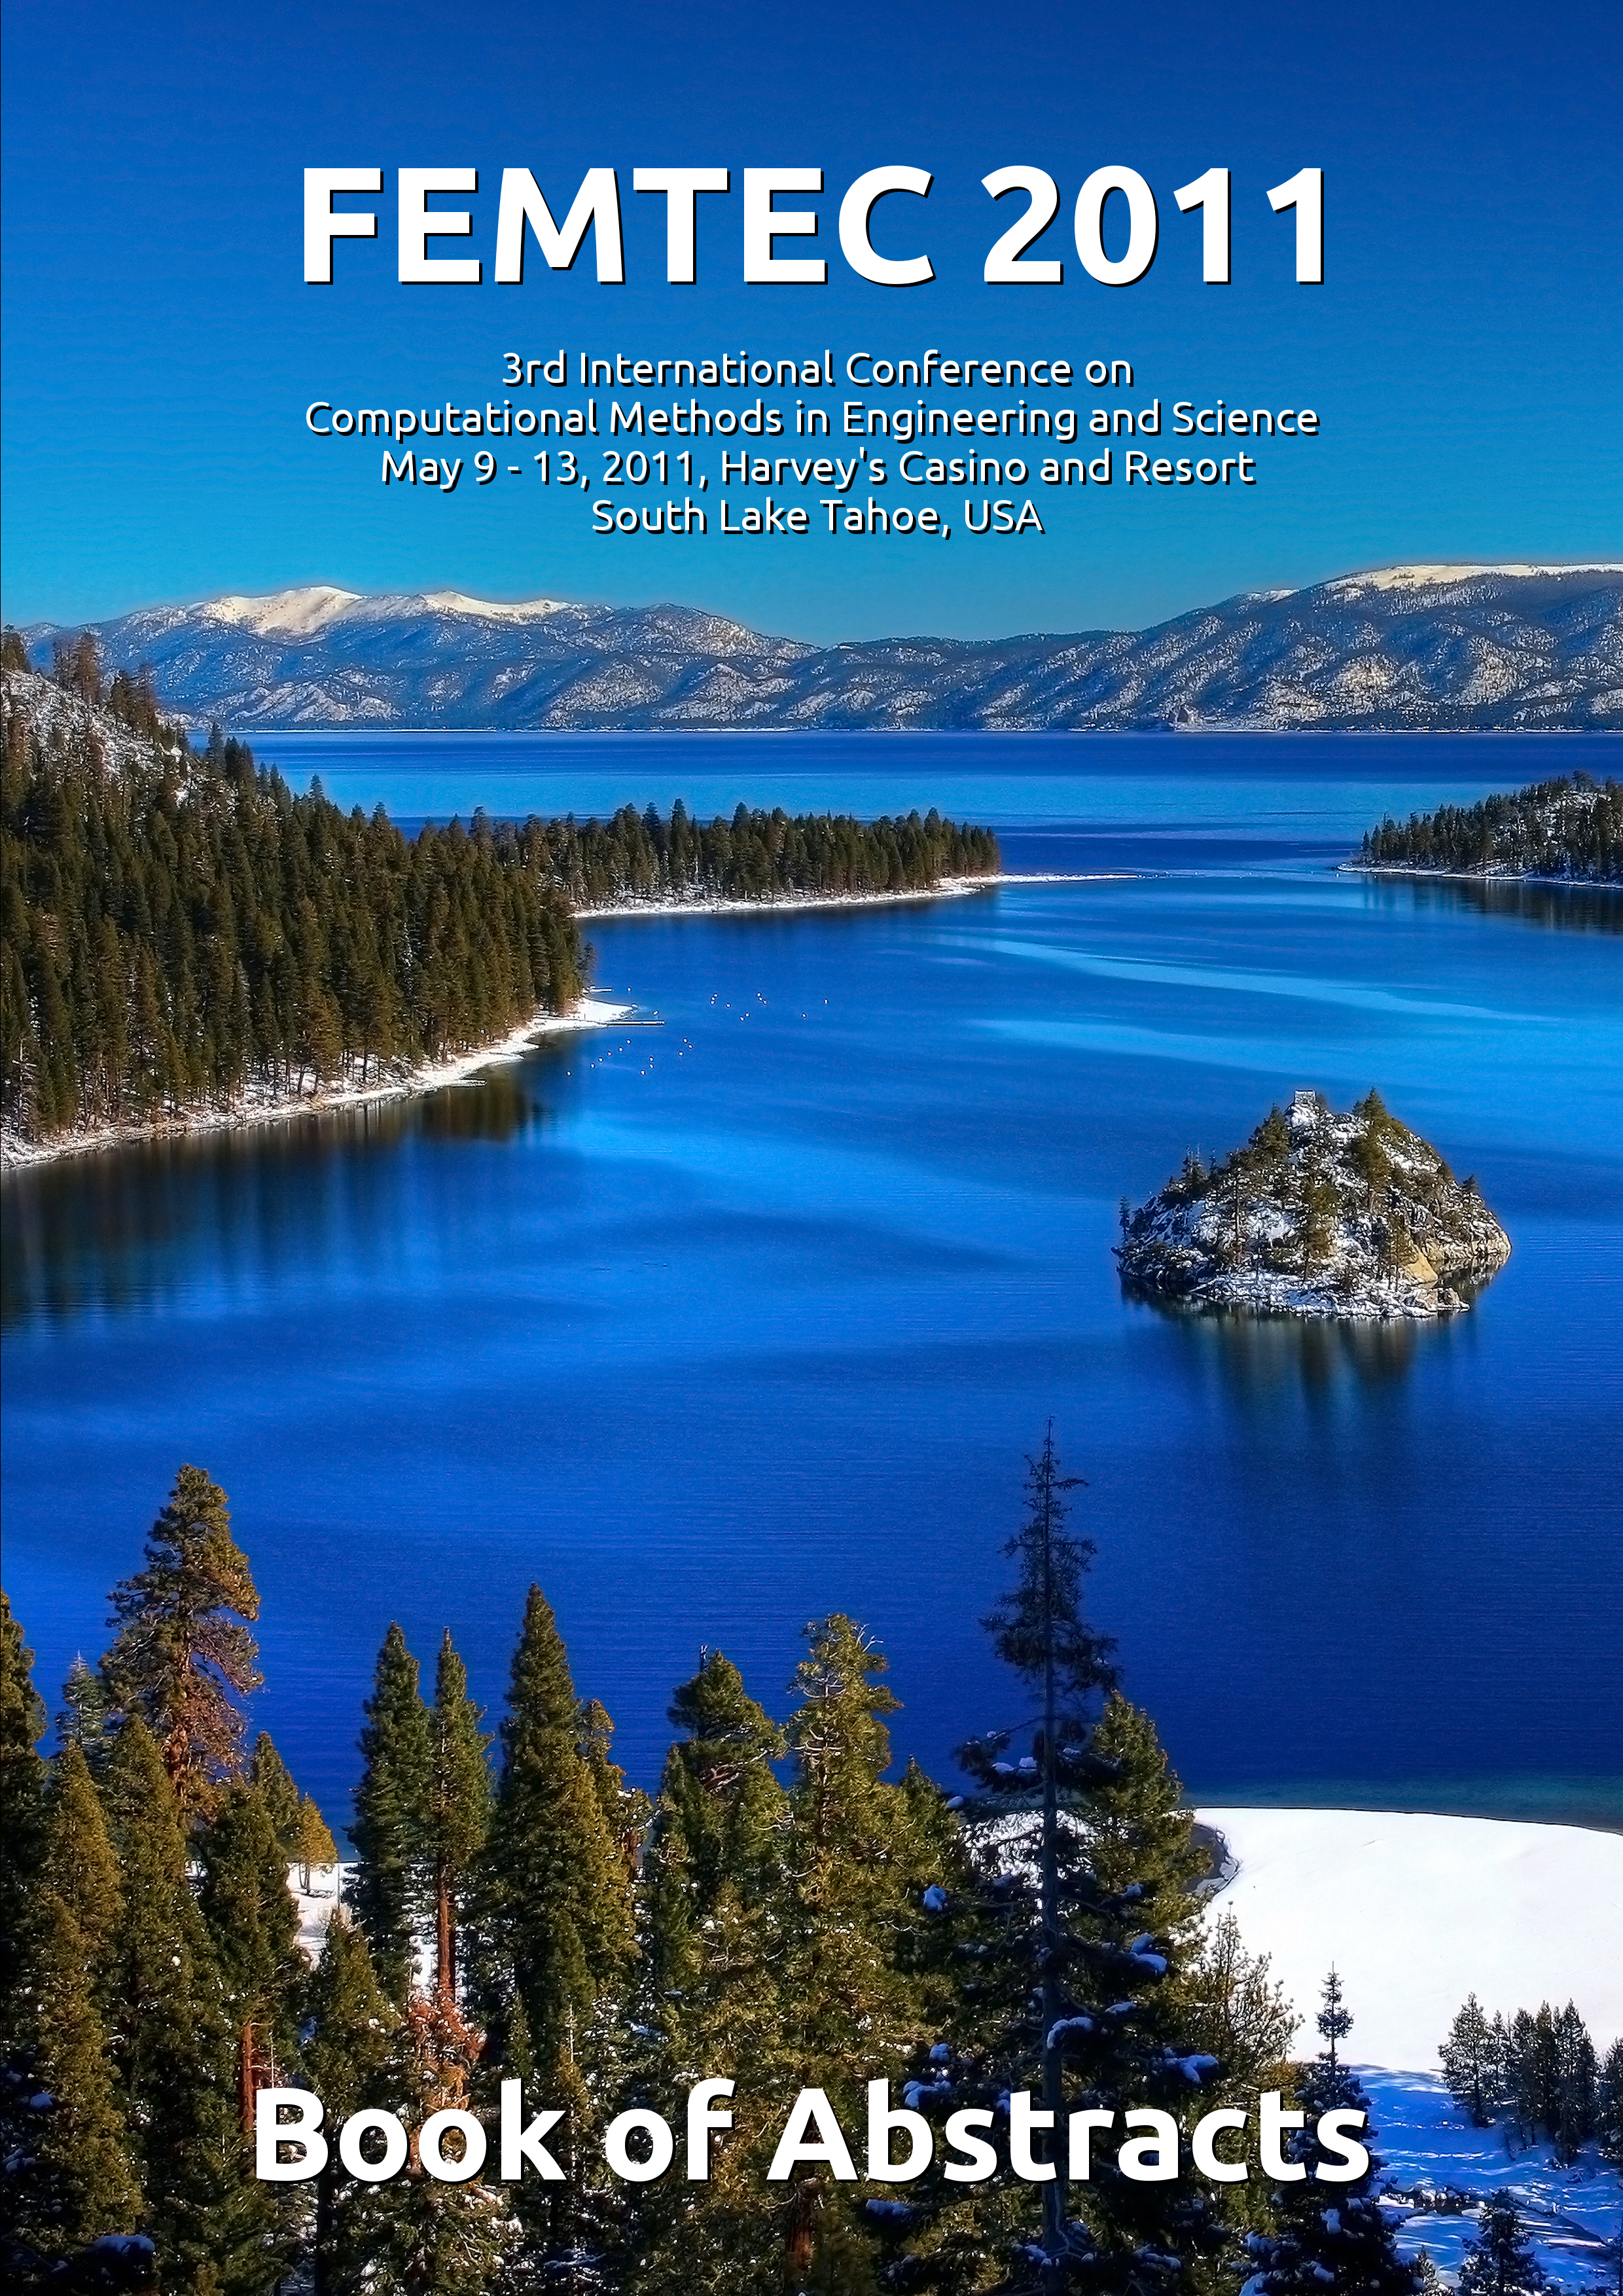
\includegraphics[width=\paperwidth,height=\paperheight]{img/background.jpg}
\vfill
}}}

\begin{document}

% INPUTTING BACKGROUND IMAGE
\AddToShipoutPicture{\BackgroundPic}
\vbox{}
\pagestyle{empty}
\newpage
\textwidth=15.5cm
\ClearShipoutPicture
\newpage


\section*{}
\small
\subsection*{About NCLab}
Networked Computing Laboratory (NCLab) is a popular Internet-based framework for 
programming, mathematics, computer modeling, 
and scientific computing. It serves students, instructors, researchers, and the general 
public. NCLab can be used free of charge for personal non-commercial purposes such as 
private hobby or self-education, as well as for individual non-funded academic research.
All other use is subject to {\bf purchasing a license} for a symbolic fee. The fees are as low as 
\$1 per user per month for educational use, and they are used to support the development 
and operational expenses. NCLab is a product of FEMhub Inc. The name "NCLab" is 
registered with the U.S. Patent and Trademark Office (USPTO) under Trademark No. 85420518.

\subsection*{Terms of Use and Pricing}
More details on purchasing a license and using NCLab are provided in the online documents 
{\bf Pricing} and {\bf Terms of Use} that are accessible from NCLab's home page 
{\tt http://nclab.com}.

\subsection*{Contact Information}
General inquiries: {\tt info@femhub.com}\\
Sales: {\tt sales@femhub.com}\\
NCLab support: {\tt support@nclab.com}\\
Agros \& Hermes support: {\tt support@femhub.com}\\
Web page: {\tt http://femhub.com}\\
{Physical address}\\
FEMhub Inc.\\
5490 Twin Creeks Dr.\\
Reno, NV 89523

\subsection*{About This Publication}
This publication can be copied and distributed without any restrictions
as long as reference to NCLab and FEMhub Inc. is preserved.

\subsection*{Acknowledgement}
This publication was created with the help of numerous freely 
available web resources and tutorials related to Python, Scipy,
Numpy, Pylab, Matplotlib, Sympy and other projects.

\normalsize

\newpage
%{\ }
\setcounter{tocdepth}{2}
\tableofcontents
%\pagestyle{plain}

\newpage

\pagestyle{plain}
\setcounter{page}{1}

\section{The {\em Cloud} is Coming. Should I Stay or Should I Run?}

You should stay. Cloud Computing sounds like a rocket science, but it is not,
and it really changes things for the better. Chances are that you are using 
it already, without even noticing it. For example, if you are using Gmail, 
Hotmail, Yahoo or another such provider to do your emails, then your data are 
stored on the cloud. 

\subsection{Some Trivia}

In the IT sense of the word, and with a bit of simplification, the {\em Cloud} 
is a pool of interconnected computers. They come in different sizes depending on the provider - 
large cloud facilities have millions of computing cores but some companies are running 
their own private clouds with relatively few computers. The computers in large clouds
are not very similar to your desktop PC -- they are stripped off many unnecessary 
things, compacted, and interconnected into a powerful grid. Their processors 
typically contain multiple {\em computing cores} that can share the same memory.
Such a {\em multicore processor} is much more efficient compared to a cluster 
of single-core PCs with the same number of cores.

The main advantage of the cloud is its {\em elasticity}. Upon your request, the
provider will assemble for you a {\em virtual server} with the parameters that 
you need. Often they have predefined {\em instances}. The following is a realistic 
example (just the name of the provider was omitted):\\

\begin{center}
\begin{tabular}{|l|l|l|l|}
\hline
{\bf Small instance} & 1.7 GB of memory & 1 core & 160 GB hard disk \\
\hline
{\bf Medium instance} & 7.5 GB of memory & 4 cores & 850 GB hard disk \\
\hline
{\bf Large instance} & 15 GB of memory & 8 cores & 1690 GB hard disk \\
\hline
\end{tabular}
\end{center}

\vspace{4mm}
\noindent
Importantly - these three instances are created by grouping the same resources together 
in different ways. An instance is created within a minute or so,
and the user can upgrade or downgrade it dynamically, depending on the actual needs.
It is quite interesting to look at the prices:

\begin{center}
\begin{tabular}{|l|l|}
\hline
{\bf Small instance} &	\$0.085 per hour\\
\hline
{\bf Medium instance}&	\$0.34 per hour	\\
\hline
{\bf Large instance}&	\$0.68 per hour\\
\hline
\end{tabular}
\end{center}

\vspace{4mm}
\noindent
In particular, these low prices mean that literally anyone has access to 
a powerful computer -- that otherwise would cost many thousands of dollars -- 
for just cents per hour. This brings new wonderful opportunities into 
education at all levels.

\subsection{Software as a Service (SaaS)}

Another big change the Cloud Computing brings is in how software is handled. 
Traditionally, one would buy a software in a big box with a small CD in it, 
and install it on one's computer. This model is now being challenged by a new 
approach called {\em Software as a Service (SaaS)}. The user does not have 
to own a copy of the software physically. Instead, the software is running 
on a remote server and accessed by users over the Internet. Typically, paying 
for the access is much less expensive compared to buying the software.

\subsection{Access from Mobile Platforms}

Last but not least, since the software is running on the cloud, the user's hardware 
does not matter so much anymore. The only really important things is to be able to 
run a web browser and access the Internet. This can be done on anything between smart 
phones, tablets, netbooks, laptops, and desktop computers. 

\subsection{Some Myths}

Very often, Cloud Computing is mentioned in the context of large 
computations in science, engineering, finance, and other fields. Yes, there are many 
cloud providers and they have to show off. But in reality, the clouds are mostly
busy processing small tasks of ordinary users. In that case, you may say, a standard 
office PC should be enough. Not exactly. Once you are not in your office, for example
while traveling, it is difficult to reach your office PC and do things as usual. 
The cloud changes that -- it allows you to access your data 
from everywhere, any time. Once you get used to it, there is no way back. 

\subsection{NCLab and K-12 Education}

NCLab is an advanced Internet-based cloud computing framework that provides 
instant access to many programming, mathematics, computer
modeling, and scientific computing activities. NCLab does not have to be installed - it 
is automatically available in any classroom that has Internet access. In 
contrast to traditional educational softwares, 
users can access their accounts and work from anywhere and at any time.
Students can start a problem at school, finish the rest at home, and notify 
the instructor about the completion with one mouse click. Most importantly, 
however, NCLab invites K-12 teachers and students to discover new STEM areas
that may not have been easy for them to access before.

\newpage


\section{Getting Started}

In order to explore NCLab, first visit its home page {\tt http://www.nclab.com}.
The upper left corner features a slide show representing selected activities 
offered by NCLab. The Cloud Monitor, located under the slide show, displays 
the current load on the cluster. The User Statistics window, located in the 
lower-right corner, provides current overview of NCLab's users and their projects. 
The window above User Statistics is a WebGL tester. WebGL is a recent web-browser technology 
that enables fast 3D grafics. If you can see in your browser an image similar to 
the one in Fig. \ref{fig:outside}, then your web browser supports it. Otherwise, 
it might be a good idea to upgrade your browser to a newer version. Note:
Internet Explorer is one of few browsers which do not support WebGL. Therefore 
we recommend using Chrome, Firefox, Opera, or Safari. A~standard login dialog 
is present in the upper-right corner.

\begin{figure}[!ht]
\begin{center}
\includegraphics[width=\textwidth]{img/outside.png}
\end{center}
%\vspace{-2mm}
\caption{NCLab's home page.}
\label{fig:outside}
\end{figure}

\newpage

\subsection{Creating an Account}

In order to create a new account, click on the link "Create free account" which is next to
"Username". The following window appears:

\begin{figure}[!ht]
\begin{center}
\includegraphics[width=0.5\textwidth]{img/create-account.png}
\end{center}
%\vspace{-2mm}
\caption{Creating new account.}
\label{fig:creacc}
\end{figure}

\noindent
In this form, fill in your preferred username, email address (to be used only if you ask
us to generate a new password for you), and password twice. Nest:

\begin{itemize}
\item If you belong to an institution 
      that uses NCLab for teaching or research, you should know your institution's code. Enter it in the form, 
      along with your first and last names. Your name will be visible to an NCLab admin at that 
      institution, who will verify that you indeed belong there.
\item If you are using NCLab for your personal hobby or self-education, for activities not 
      related to any institutional use, then leave the last three lines empty. 
\end{itemize}
After clicking OK, you are ready to login!

\subsection{After Login}

Inside NCLab, you will find yourself in an environment that is similar
to the standard computer desktop. Your Groups icon will not be lighted 
green yet, such as the one in Fig. \ref{fig:desktop}. The green light 
indicates that someone in some of your Groups is currently in NCLab. 

\begin{figure}[!ht]
\begin{center}
\includegraphics[width=\textwidth]{img/desktop.png}
\end{center}
%\vspace{-2mm}
\caption{NCLab desktop after login.}
\label{fig:desktop}
\end{figure}

\noindent
More about Groups and Chat will be said in a moment. First, let us briefly 
describe the other icons:

\begin{itemize}
\item File Manager is used to manage files and folders similarly to Windows Explorer. 
\item Programming Module enables programming in Karel (popular educational language for beginners),
      Python (modern programming language for advanced applications), and Javascript 
      (most popular language for web development). Additional languages are in preparation.
\item Fractal Explorer is an interactive graphical application that allows the users
      to learn about Mandelbrot and Julia fractals, and to generate beautiful fractal art.
\item Settings: Here the user can upload his/her avatar image (to be used in Groups and Chat), 
      request a new password, and adjust sound preferences.
\item Help launches a quick help about NCLab.
\item Logoff will close all applications and end the session.
\end{itemize}

\section{Groups and Chat}

In NCLab users can form groups, see who is online, and chat in real time. In order to 
create a new group, click on the Groups icon. A window similar to the one shown 
in Fig. \ref{fig:groups} appears. This concrete screenshot shows four groups of the 
user "solin" -- the top one was created by Jordan, the other three by solin. The 
green light next to the last group indicates that someone in that group
is currently in NCLab. Before we go look who that is, notice that you can create a
new group of your own by clicking on "New Group". You can also see instantly who in your 
groups is in NCLab by clicking on "Who's online".


\begin{figure}[!ht]
\begin{center}
\includegraphics[width=0.5\textwidth]{img/groups.png}
\end{center}
%\vspace{-2mm}
\caption{Groups window, showing that someone in the last group is currently in NCLab.}
\label{fig:groups}
\end{figure}

\noindent 
After clicking on the last group, it is revealed that Emily and Rick are currently in NCLab. 

\begin{figure}[!ht]
\begin{center}
\includegraphics[width=0.5\textwidth]{img/groups-2.png}
\end{center}
%\vspace{-2mm}
\caption{Detail of the last group.}
\label{fig:groups-2}
\end{figure}

\noindent
By clicking on any user who has the green light next to him/her,
it is possible to start a chat. Or, you may be contacted first, 
of course. The Chat window is shown in Fig. \ref{fig:chat}.

\begin{figure}[!ht]
\begin{center}
\includegraphics[width=0.4\textwidth]{img/chat.png}
\end{center}
%\vspace{-2mm}
\caption{Chat window.}
\label{fig:chat}
\end{figure}


\section{Using NCLab as a Calculator}

The advantage of simple calculators, such as the one shown in Fig. \ref{fig:xcalc}
is that they only have a few functions, and thus can be operated using a few buttons.

\begin{figure}[!ht]
\begin{center}
\includegraphics[width=0.4\textwidth]{img/xcalc.png}
\end{center}
%\vspace{-2mm}
\caption{Simple calculator.}
\label{fig:xcalc}
\end{figure}
\noindent
Compared to this calculator, NCLab provides an enormous functionality 
that would require thousands of buttons. So instead of buttons,
in NCLab we use simple commands to get the results we want. This is 
easy and fun, let's try it.

We begin with clicking on the File Manager icon. which launches the File 
Manager. Next go to the menu Project in the upper-left corner. There go 
through the submenu New to Python and click. This will lanuch a new Python 
project, as illustrated in Fig. \ref{fig:python}. 

\newpage

\begin{figure}[!ht]
\begin{center}
\includegraphics[width=\textwidth]{img/python.png}
\end{center}
%\vspace{-2mm}
\caption{Python project.}
\label{fig:python}
\end{figure}
\noindent
For now we will be using Python for simple math operations only,
but you could start writing an advanced Python program right 
here if you wanted. An introduction to the Python programming 
language is the subject of another NCLab tutorial.

Before we begin, it is a good idea to save your project under some 
name. This is done through the menu File and submenu Save. For 
now we can save the project in the base folder. Later you can create 
a new folder through the File Manager's menu Folder, and drag there
the project by mouse, to keep your data organized.

\subsection{Simple Arithmetic}

Your project now contains a single {\em input cell}. Let's write 
something simple into it, for example "1 + 2", and click 
the link "run" right under the input cell. This sends a request to 
the cloud, and an answer comes back immediately. It is displayed 
in a new (yellow) {\em output cell}, as shown in Fig. \ref{fig:1p3}.

\newpage
\begin{figure}[!ht]
\begin{center}
\includegraphics[width=\textwidth]{img/1p3.png}
\end{center}
%\vspace{-2mm}
\caption{Evaluating the expression "1+2".}
\label{fig:1p3}
\end{figure}
\noindent
\noindent
In addition to input and output cells, you can use {\em text cells}
to keep your project commented. This is strongly recommended. In
order to add a new text cell above the input cell, click into
the input cell, and then in menu Edit choose "New text cell above
active cell". A new text cell appears, asking you to click there to
edit its contents. Do so, and write, for example, "**Adding numbers**".
The double stars are used to make a text between them bold face. 
Then click on the link "save" right under the text cell. The result 
is shown in Fig. \ref{fig:1p3r}.

\newpage
\begin{figure}[!ht]
\begin{center}
\includegraphics[width=\textwidth]{img/1p3r.png}
\end{center}
%\vspace{-2mm}
\caption{New descriptive text cell was added above the input cell.}
\label{fig:1p3r}
\end{figure}
\noindent
\noindent
If you like, you can click back into the input cell, change 
the numbers, and click the "run" link under the cell again. 
This will send a new request to the cloud and after the answer 
comes back, the result will be displayed in the existing output 
cell. 

Let's continue by creating a new empty input cell. To do this, click
into the previous input cell, and in menu Edit choose "New input cell 
below active cell". The new input cell will appear below the yellow 
output cell (it will never be placed between an input cell and its 
result). In there, we can experiment with other arithmetic operations 
including subtraction (try for example "5 - 3"), multiplication 
(try for example "3.21 * 7.45"). The results are shown in Fig. \ref{fig:1p3r2}.

\newpage
\begin{figure}[!ht]
\begin{center}
\includegraphics[width=\textwidth]{img/1p3r2.png}
\end{center}
%\vspace{-2mm}
\caption{Subtraction and multiplication.}
\label{fig:1p3r2}
\end{figure}
\noindent
At this point we may go to menu Edit and click on 
"Remove all output" -- this will free up some space.

\subsection{Division of Two integers Always is an Integer}

Numbers such as "12" or "5" are integers. In Python, as well as 
in other major programming languages, the {\bf result of division of 
two integers always is an integer}. This means that anything beyond 
the decimal point in the result is erased! Let us see this in reality:

\newpage
\begin{figure}[!ht]
\begin{center}
\includegraphics[width=\textwidth]{img/div1.png}
\end{center}
%\vspace{-2mm}
\caption{Division of two integers always is an integer \& two ways to make division safe.}
\label{fig:div1}
\end{figure}
\noindent
Fig. \ref{fig:div1} shows that evaluating simply 12/5 leads to a wrong result. An easy fix is 
to convert one of the numbers into a float by appending a decimal point to it. Still
another way, also shown in  Fig. \ref{fig:div1}, is to convert one of the numbers into a float 
via the function {\tt float()}. The latter approach works even for the division of variables "a/b"
where one may not know exactly whether they are integers or floats. Whenever at least 
one of the numbers if float, the result is a float. \\

\noindent
If you are a mathematician -- yes, you are right. we forgot to discuss division by zero. 
It is useful to see how NCLab reports errors, so let's do it!

\newpage
\begin{figure}[!ht]
\begin{center}
\includegraphics[width=\textwidth]{img/divzero.png}
\end{center}
%\vspace{-2mm}
\caption{Error is reported when dividing by zero.}
\label{fig:divzero}
\end{figure}
\noindent
Since the error message in Fig. \ref{fig:divzero} mentioned modulo, we added there one more 
input cell demonstrating how modulo is done -- using the \% symbol.

\subsection{Using Simple Functions}

In order to calculate square roots, exponentials, sins, cosins, tangents, and all other 
simple functions, the best way is to import Numpy as shown in Fig. \ref{fig:fns}. Numpy is a standard Python library for
numerical computations.
For a complete overview of functions provided by Numpy we recommend the 
web page {\tt http://www.scipy.org/Numpy\_Functions\_by\_Category}.

\newpage
\begin{figure}[!ht]
\begin{center}
\includegraphics[width=\textwidth]{img/fns.png}
\end{center}
\vspace{-4mm}
\caption{Using elementary functions.}
\label{fig:fns}
%\vspace{-6mm}
\end{figure}
\noindent

\section{Plotting Functions of One Variable}

Plotting can be done via the Pylab library. Pylab is a standard Python library that is 
superior in almost every way to MATLAB (expensive commercial product whose usage is 
quite similar to what we are doing here). Concretely, plotting is illustrated in Fig. \ref{fig:plot}.

\begin{figure}[!ht]
\begin{center}
\includegraphics[width=\textwidth]{img/plot.png}
\end{center}
\vspace{-2mm}
\caption{Plotting functions of one variable.}
\label{fig:plot}
\vspace{-1cm}
\end{figure}
\newpage
The plot can be made fancier by adding a label, and also the color 
and the line style can be changed, as shown in Fig. \ref{fig:plot2}.

\begin{figure}[!ht]
\begin{center}
\includegraphics[width=\textwidth]{img/plot2.png}
\end{center}
\vspace{-2mm}
\caption{Adding labels, and changing colors and line styles.}
\label{fig:plot2}
\end{figure}
\noindent
While the label definition is probably clear, let us give some more examples 
of colors and line styles:

\begin{itemize}
\item "b-"... continuous blue line
\item "b."... blue line consisting of small dots
\item "bo"... blue line consisting of big dots
\item "r-"... continuous red line
\item "r."... red line consisting of small dots
\item "ro"... red line consisting of big dots
\end{itemize}
For a complete list of options, please visit the Pylab page {\tt http://www.scipy.org/PyLab}.



\section{Algebra}

To be continued...

\subsection{Expansion}

TBC

\section{Calculus}

TBC



\section{Differential Equations}

TBC


\section{Advanced 3D Plotting}

\end{document}
